\documentclass[12pt,oneside,final]{thesis}

\usepackage[superscript]{cite}
\usepackage{amsmath,amsfonts}
\usepackage{graphicx}
\graphicspath{{./figs/}}
\usepackage{fixltx2e}
\usepackage{array}
% wrapfig is fragile: use sparingly
\usepackage{wrapfig} 
%\usepackage{times}  % Use this for ugly fonts

\usepackage{upgreek}
\usepackage{hyperref}
\usepackage{setspace}

\usepackage{booktabs}
\usepackage{multirow}
\usepackage{longtable}
\usepackage[font=singlespacing, labelfont=bf]{caption}
%\usepackage{CV}

\usepackage{enumitem}
\newlist{inlinelist}{enumerate*}{1}
\setlist*[inlinelist,1]{%
  label=(\arabic*),
}

\usepackage{fancyhdr}    % Use nice looking headers along with the required footer page numbers   
%\usepackage[hypertex]{hyperref}
%---------------------------------------------added by JYao--------------------------
\usepackage[para,online,flushleft]{threeparttable}
\usepackage{natbib}
\usepackage{caption}
\usepackage{subcaption}
\usepackage{float}
\usepackage[usenames,dvipsnames]{xcolor}
\usepackage{color, colortbl}
\usepackage{lscape}
%-------------------------------------------------------------------------------------------


%Define the header/footer style
\pagestyle{fancy}
\fancyhf{}
\setlength{\headheight}{15pt}
\lhead{\leftmark}
\cfoot{\thepage}
\renewcommand{\headrulewidth}{0pt}
\fancypagestyle{plain}{% Redefine ``plain'' style for chapter boundaries
\fancyhf{} % clear all header and footer fields
\fancyfoot[C]{\thepage} % except the center
\renewcommand{\headrulewidth}{0pt}
\renewcommand{\footrulewidth}{0pt}}

%\tolerance=10000

%\makeglossary % enable the glossary

%-----------------------------------added by JYao-----------------------------------
\def\newblock{\hskip .11em plus .33em minus .07em}
\def\keywordname{{\bfseries Keywords}}
\def\keywords#1{\par\addvspace\medskipamount{\rightskip=0pt plus1cm
\def\and{\ifhmode\unskip\nobreak\fi\ $\cdot$
}\noindent\keywordname\enspace\ignorespaces#1\par}}
%
\def\JELname{{\bfseries JEL Classification}\enspace}
\def\JEL#1{\par\addvspace\medskipamount{\rightskip=0pt plus1cm
\def\and{\ifhmode\unskip\nobreak\fi\ $\cdot$
}\noindent\JELname\ignorespaces#1\par}}

\def\Advisorname{{\bfseries Advisors}\enspace}
\def\Advisors#1{\par\addvspace\medskipamount{\rightskip=0pt plus1cm
\def\and{\ifhmode\unskip\nobreak\fi\ $\cdot$
}\noindent\Advisorname\ignorespaces#1\par}}

\begin{document}

\title{ESSAYS ON CONSUMPTION }
\author{Edmund Crawley}
\degreemonth{May}
\degreeyear{2018} 
\dissertation
\doctorphilosophy
\copyrightnotice


% add your chapters, best way is to have separate TeX files for each chapter
%%% FRONTMATTER
\begin{frontmatter}

% generate title
\maketitle

\begin{abstract}

Abstract goes here.

\vspace{1cm}

\keywords{Consumption, Marginal Propensity to Consume, Heterogeneity}

\JEL{D12}

\Advisors{\\ Professor Christopher Carroll\\ Professor Jon Faust\\ Professor Jonathan Wright}


\end{abstract}

\begin{acknowledgment}

Thanks!

\end{acknowledgment}

\begin{dedication}
 
This thesis is dedicated to \ldots

\end{dedication}

% generate table of contents
\tableofcontents

% generate list of tables
\listoftables

% generate list of figures
\listoffigures

\end{frontmatter}

%\chapter{Time Aggregation in Panel Data on Income and Consumption}

\section{Abstract}
In 1960 Working noted that time aggregation of a random walk induces serial correlation in the first differences that is not present in the original series. This important contribution has been overlooked in a large recent literature analyzing income and consumption in panel data. This paper takes \cite{blundell_consumption_2008} as an example and shows how to correct for this problem. I find the estimate for the partial insurance to transitory shocks, originally estimated to be 5\%, is equal to 24\% when corrected for time aggregation. This estimate is much closer to estimates from the literature that uses natural experiments to estimate the marginal propensity to consume out of transitory shocks.

\section{Introduction}
In a short note in Econometrica, \cite{working_note_1960} made the simple but important point that time aggregation can induce serial correlation that is not present in the original series. This fact was readily absorbed by the macroeconomic literature, where such time aggregated series are common (for an example see \cite{campbell_consumption_1989}). Recently, by studying the covariance structure of panel data, much progress has been made in understanding household income and consumption dynamics. However, this literature has not accounted for the serial correlation induced by the time aggregated nature of observed income and consumption data. This oversight can result in significant bias. This paper will focus on the implications of time aggregation for the methodology in \cite{blundell_consumption_2008} (henceforth BPP), but it applies to a broad swath of the literature. I show that the pass through from transitory income to consumption, originally estimated by BPP to be 5\%, is close to 25\% when the serial correlation in the data induced by time aggregation is accounted for.

\subsection{What is Time Aggregation?}
Many observed time series in economics are given at a lower frequency than the underlying data that generates them. For example, income is often observed at an annual frequency when it may in fact consist of paychecks arriving at a monthly, biweekly or irregular timetable. To transform income into an annual frequency we sum up all the income that was received by a household during the year, a process known as time aggregation. The key insight of \cite{working_note_1960} is that even if there is no correlation between changes in income at the underlying frequency, the resulting time aggregated series will show positive autocorrelation. The intuition behind this can be seen in figure \ref{fig:TimeAggExample} showing an income process that begins at zero and increases to one in the second year. The top left graph shows the path of income if the shock occurs exactly at the start of the second year, and the bottom left graph shows the time aggregated process exactly mirrors that. There is no income in the first year and one unit of income in each of the second and third years. The top right shows an alternative income process in which the shock occurs half way through the second year. Now the resulting time aggregated process (bottom right) does not mirror the underlying. As before there is no income in the first year, but in the second year the individual receives an income of one for half the year, resulting in a time aggregated income of 0.5. In the third year the individual receives an income of one for the entire year, and hence a time aggregated income of one. If we can only see the time aggregated process, when we observe income increasing from year one to year two we do not know if the shock occurred at the beginning of the year or half way through. If it occurred at the beginning of the year, as in the left hand graphs of figure \ref{fig:TimeAggExample}, then we would not expect to see any further increase in the time aggregated process associated with it. However, if it occurred half way through, as in the right hand graphs of figure \ref{fig:TimeAggExample}, we would only have observed half the total increase in income and would expect the time aggregated process to continue to increasing in the following period. Therefore, assuming there is some positive probability that the shock occurred half way through the second period, we would expect to see further increases in the observed process. This is how time aggregation induces serial correlation in the first difference of an observed process even when the underlying process is a random walk. Section \ref{TimeAggRandomWalk} lays this out formally and shows that this autocorrelation tends to $\frac{1}{4}$ as the number of time subdivisions increases to infinity.
\begin{figure}
	\caption{Time Aggregation Induces Serial Correlation}
	\label{fig:TimeAggExample}
	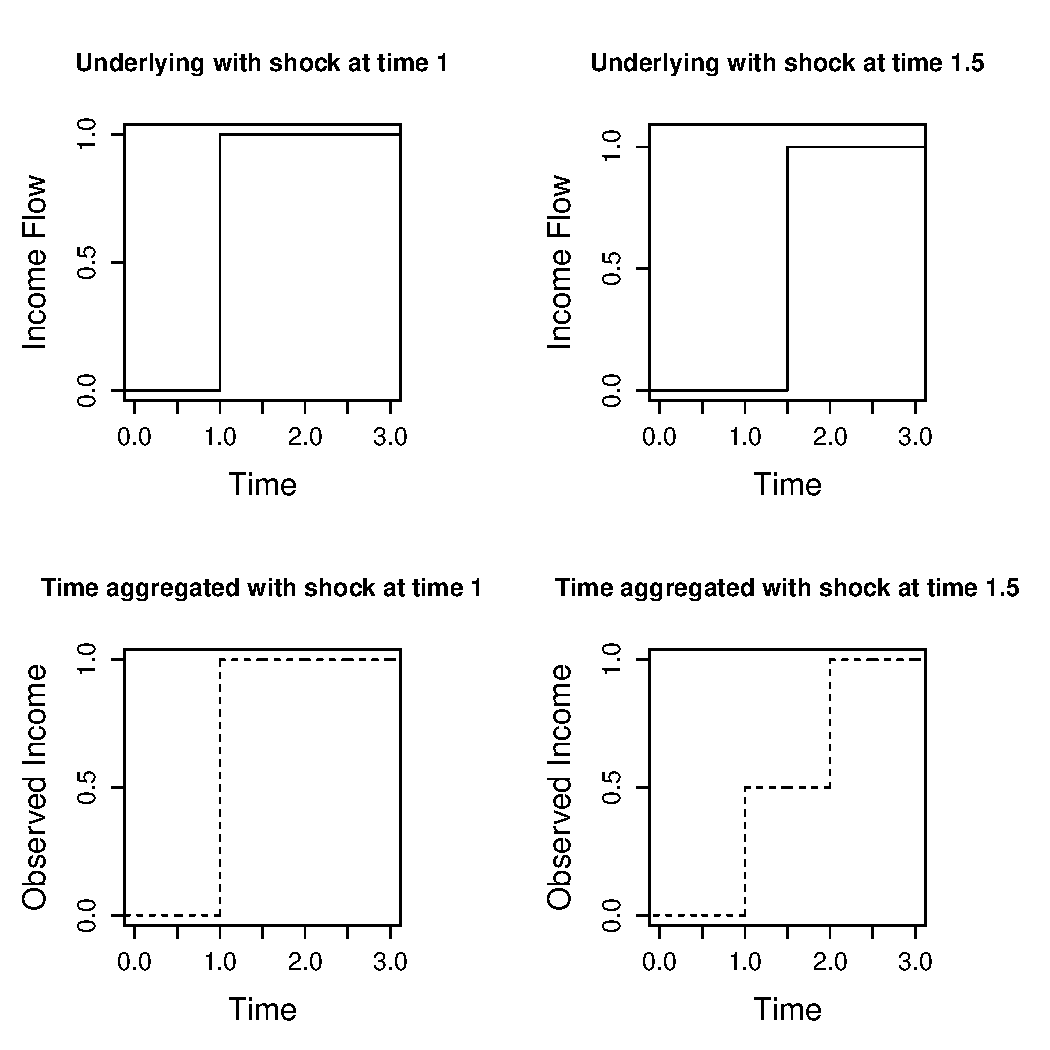
\includegraphics[width=1\textwidth]{./Chapter1/Figures/TimeAggExample.pdf}
\end{figure}

%NEED TO SPEND TIME CONNECTING THIS WITH THE LITERATURE
%\subsection{Relation to the Literature}

\section{Time Aggregated Random Walk} \label{TimeAggRandomWalk}
I this section I formally prove that a time aggregated random walk is autocorrelated and show that this autocorrelation tends to $\frac{1}{4}$ as the number of time subdivisions increases to infinity. I will also introduce continuous time notation that will be used for the underlying model in section \ref{BPP}.

\subsection{The two sub-division case}
I begin with the two-subdivision case. The underlying income process follows a random walk at discrete time periods $t\in \{0,1,2,3,...\}$:
\begin{align*}
y_t = \begin{cases}
0 \qquad & \text{if } t=0\\
y_{t-1} + \varepsilon_t & \text{otherwise}
\end{cases}
\end{align*}
where $\varepsilon_t$ is i.i.d. and has variance $\sigma^2$. The  time aggregated process is observed every two periods at $T\in\{2,4,6,...\}$ and is equal to the sum of income over the two periods leading up to it:
\begin{align*}
y_T^{obs} = y_T + y_{T-1}
\end{align*}
The observed income change is given by:
\begin{align*}
\Delta^2 y_T^{obs} &= y_T^{obs} - y_{T-2}^{obs} \\
&= \varepsilon_T + 2\varepsilon_{T-1} + \varepsilon_{T-2}
\end{align*}
This allows for easy calculation of the serial correlation:
\begin{align*}
\mathrm{Cov}(\Delta^2 y_T^{obs},\Delta^2 y_{T-2}^{obs}) &= \sigma^2 \\
\mathrm{Var}(\Delta^2 y_T^{obs}) &= \sigma^2 + 4\sigma^2 + \sigma^2 \\
&= 6\sigma^2 \\
\mathrm{Corr}(\Delta^2 y_T^{obs},\Delta^2 y_{T-2}^{obs}) &= \frac{1}{6}
\end{align*}

\subsection{The N sub-division case}
The two sub-division case easily extends to N sub-divisions. Using the same underlying income process, the observable income process is now aggregated over N periods:
\begin{align*}
y_T^{obs} = \sum_{t=T-N+1}^{T} y_t
\end{align*}
So that the observed change in income is:
\begin{align*}
\Delta^N y_T^{obs} &= \sum_{t=T-N+1}^{T} y_t - y_{t-N} \\
&= \varepsilon_T + \varepsilon_{T-1} +  \qquad...  \qquad+ \varepsilon_{T-N+2} + \varepsilon_{T-N+1} \\
& \qquad \   +  \varepsilon_{T-1} + \varepsilon_{T-2}  + \qquad...  \qquad \quad \ + \varepsilon_{T-N+1} + \varepsilon_{T-N} \\
& \qquad \qquad  \quad \ \, +  \varepsilon_{T-2} + \varepsilon_{T-3} + \qquad ... \\
& \qquad \qquad \qquad \qquad \qquad \qquad ...\\
& \qquad \qquad \qquad \qquad \qquad \qquad \qquad \qquad \ +  \varepsilon_{T-N+1} +\qquad ...  \qquad + \varepsilon_{T-2N+2} \\
&= N \varepsilon_{T-N+1} + \sum_{i=1}^{N-1} i\Big(\varepsilon_{T-i+1} + \varepsilon_{T-2N+i+1} \Big)
\end{align*}
We can now calculate the autocorrelation:
\begin{align*}
\mathrm{Cov}(\Delta^N y_T^{obs},\Delta^N y_{T-N}^{obs}) &=\sum_{i=1}^{N-1} i(N-i) \sigma^2 \\
&=  \frac{N(N^2-1)}{6} \sigma^2 \\
\mathrm{Var}(\Delta^N y_T^{obs}) &= N^2\sigma^2 + 2\sum_{i=1}^{N-1} i^2 \sigma^2 \\
&= \frac{N(2N^2+1)}{3}\sigma^2 \\
\mathrm{Corr}(\Delta^N y_T^{obs},\Delta^N y_{T-N}^{obs}) &= \frac{N^2-1}{2(2N^2+1)} \rightarrow \frac{1}{4} \text{ as } N \rightarrow \infty
\end{align*}
\subsection{The Continuous Time Case} \label{cont_time_case}
It will turn out to be significantly simpler to work with a model in which shocks can occur at any point in continuous time. Here I introduce some notation for such a model, and show that it gives a good approximation even if the actual underlying process is discrete (say quarterly or monthly).

The underlying income process will be modeled as a martingale process in continuous time, $y_t$, where for all  $s_1>s_2>s_3>s_4>0$:
\begin{align*}
\mathrm{Var}(y_{s_1}-y_{s_2})=(s_1-s_2)\sigma^2 \\
\mathrm{Cov}(y_{s_1}-y_{s_2},y_{s_3}-y_{s_4}) = 0 \\
y_s = 0 \qquad \text{if } s<0
\end{align*}
The process has independent increment increments. A Brownian motion would satisfy these criteria, but although in continuous time there is no restriction that it is a continuous process (it may have jumps).\footnote{Note that such a process will take both positive and negative values, and therefore may not be a good choice for an income process. In appendix \ref{log_tranformation}, by looking at the limit of discrete time models with m sub-periods, I show that under certain assumptions the same results approximately hold when shocks are multiplicative rather than additive.} The observed income process is the sum of income over a year:
\begin{align*}
\bar{y}_T &= \int_{T-1}^{T} y_t dt \\
&= \int_{T-1}^{T} \int_{0}^{t} dy_s dt 
\end{align*}
So that:
\begin{align*}
\Delta \bar{y}_T &= \int_{T-1}^{T} \int_{0}^{t} dy_s dt - \int_{T-2}^{T-1} \int_{0}^{t} dy_s dt \\
&= \int_{T-1}^{T} \int_{t-1}^{t} dy_s dt \\
&= \int_{T-1}^{T} (T-s) dy_s + \int_{T-2}^{T-1} (s-(T-2)) dy_s 
\end{align*}
The autocorrelation can now be calculated:
\begin{align*}
\mathrm{Cov}(\Delta \bar{y}_T,\Delta \bar{y}_{T-1}) &=  \int_{T-2}^{T-1} (T-1-s)(s-(T-2)) \sigma^2 dt \\
&= \frac{1}{6}\sigma^2 \\
\mathrm{Var}(\Delta \bar{y}_T) &= \int_{T-1}^{T} (T-s)^2 \sigma^2 dt + \int_{T-2}^{T-1} (s-(T-2))^2 \sigma^2 dt \\
&= \frac{2}{3}\sigma^2 \\
\mathrm{Corr}(\Delta \bar{y}_T,\Delta \bar{y}_{T-1}) &= \frac{1}{4}
\end{align*}
Which is unsurprisingly the same as the limit of the autocorrelation in the N sub-periods case.
\begin{figure}
	\caption{Induced Autocorrelation for different N}
	\label{fig:InducedAutocorrelation}
	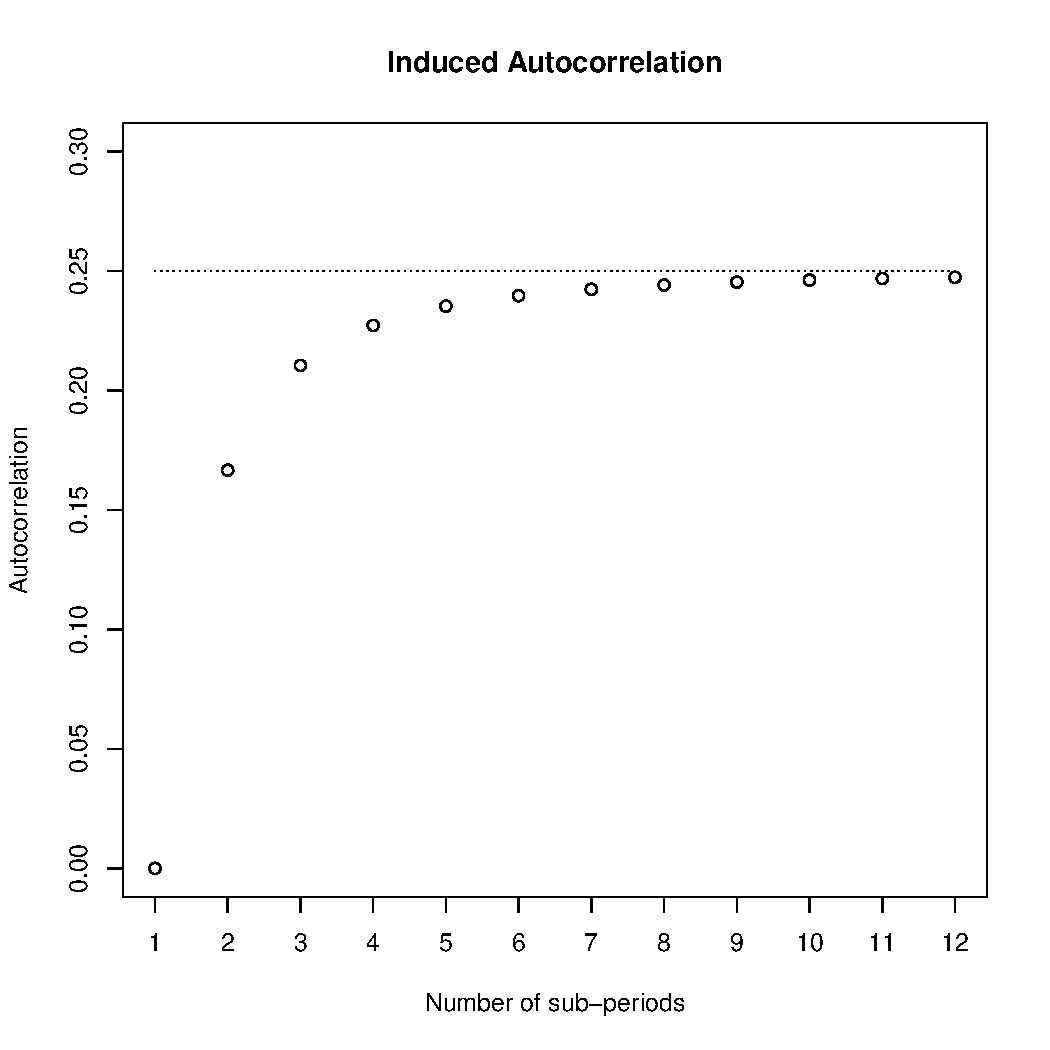
\includegraphics[width=1\textwidth]{./Chapter1/Figures/InducedAutocorrelation.pdf}
\end{figure}
Figure \ref{fig:InducedAutocorrelation} shows how fast the N sub-period case converges towards the continuous time case. When $N=1$ the time aggregated process is the same as the underlying random walk so the autocorrelation is zero. When income is quarterly ($N=4$) the autocorrelation is 0.23 and is closely approximated by the continuous time model. With monthly ($N=12$) or higher frequency for income shocks the discrete and continuous models are almost indistinguishable. 

\section{Time Aggregation in \cite{blundell_consumption_2008}} \label{BPP}
I will focus on the methodology for estimating partial ``insurance'' coefficients to transitory and permanent shocks introduced by \cite{blundell_consumption_2008}. I choose this paper both because it provides a clear example where time aggregation biases the results quantitatively, and also because the methodology has become common place in the literature and could now be considered a workhorse model. Indeed \cite{kaplan_how_2010} state in their paper that applies the method to simulated data that ``we argue that the BPP insurance coeffcients should become central in quantitative
macroeconomics"

\subsection{The Model in Discrete Time Without Time Aggregation}
Here I briefly describe the method followed by \cite{blundell_consumption_2008}. For more detail please refer to their original paper. The core of the model are their assumptions on the income and consumption processes. The model described here is a simplified version of the original in order to highlight the role played by time aggregation.\footnote{In this simplified model I assume insurance parameters are constant accross both time and households, that the transitory component of income has no persistence, and that there are no taste shocks. These elements are reintroduced in section \ref{evidence} in which I show the quantitative effect of time aggregation.} 

Unexplained log income growth for household $i$ follows the process:
\begin{align*}
\Delta y_{i,t} = \zeta_{i,t} + \Delta \nu_{i,t}
\end{align*}
where $\zeta_{i,t}$ (the change in permanent income) and $\nu_{i,t}$ (transitory income) are each i.i.d. and independent of each other. The variance of permanent shocks ($\sigma^2_{\zeta}=\mathrm{Var}(\zeta_{i,t})$) and transitory shocks ($\sigma^2_{\nu}=\mathrm{Var}(\nu_{i,t})$) will be of interest. These variances can be identified from observable data by noting the following identities (where the household identifier $i$ has been removed for clarity):
\begin{align}
\sigma^2_{\zeta}&=\mathrm{Var}(\zeta_{t}) \nonumber \\
&= \mathrm{Cov}(\Delta y_{t}, \Delta y_{t-1}+\Delta y_{t}+\Delta y_{t+1}) \label{perm_var}\\
\sigma^2_{\nu}&=\mathrm{Var}(\nu_{t}) \nonumber \\
&= -\mathrm{Cov}(\Delta y_{t},\Delta y_{t+1}) \label{tran_var}
\end{align}
The unexplained change in log consumption is modeled as a random walk that moves in response to changes in both permanent income and transitory income:
\begin{align*}
\Delta c_{i,t} = \phi \zeta_{i,t} + \psi \nu_{i,t} 
\end{align*}
where $\phi$ and $\psi$ are the \textit{partial insurance} parameters for permanent and transitory shocks respectively. A value of zero implies full insurance (consumption does not respond at all to the income shock), while a value of one implies no insurance. These insurance parameters can be identified in the data from these identities:
\begin{align}
\phi&= \frac{\mathrm{Cov}(\Delta c_{t}, \Delta y_{t-1}+\Delta y_{t}+\Delta y_{t+1})}{\mathrm{Cov}(\Delta y_{t}, \Delta y_{t-1}+\Delta y_{t}+\Delta y_{t+1})} \label{phi}\\
\psi&= \frac{\mathrm{Cov}(\Delta c_{t},\Delta y_{t+1})}{\mathrm{Cov}(\Delta y_{t},\Delta y_{t+1})} \label{psi}
\end{align}
It is useful to think of equations \ref{phi} and \ref{psi} as IV regressions of consumption growth on income growth where (\ref{phi}) uses income growth over 3 periods as an instrument to identify permanent shocks, while (\ref{psi}) uses income growth in the following period to identify transitory shocks (a transitory shock to income today predicts that income will go down by the same amount in the following period).

The four equations \ref{perm_var}, \ref{tran_var}, \ref{phi} and \ref{psi} are the core of the BPP identification methodology. In the following section I will show how this identification fails when time aggregation is accounted for.

\subsection{The Model in Continuous Time with Time Aggregation}
The model in this section will be the exact analog of the discrete time BPP model just described, but embedded in continuous time where shocks are spread uniformly throughout the year.\footnote{There is little formal evidence on the distribution of shocks throughout the year. While this assumption is unlikely to be strictly true, it is more reasonable that the implicit assumption of BPP that shocks all occur 1st January each year.} For the income process we will assume two underlying martingale processes (possibly with jumps), $P_t$ and $Q_t$ such that for all $s_1>s_2>s_3>s_4>0$:
\begin{align*}
\mathrm{Var}(P_{s_1}-P_{s_2})=(s_1-s_2)\sigma_P^2 \\
\mathrm{Cov}(P_{s_1}-P_{s_2},P_{s_3}-P_{s_4}) = 0 \\
P_s = 0 \qquad \text{if } s<0
\end{align*}
and similarly for $Q_t$.  Instantaneous income in a period $dt$ is given by:\footnote{A more formal treatment of how to relate this to the log income process is given in appendix \ref{log_tranformation}}
\begin{align}
dy_t = \Big( \int_{0}^{t}dP_s \Big) dt  +dQ_t \label{income_process}
\end{align}
that is they receive their permanent income ($P_t =\int_{0}^{t}dP_s $) flow multiplied by time $dt$ in addition to a one-off transitory income $dQ_t$.

Keeping with the assumption that consumption is a random walk with insurance parameters $\phi$ and $\psi$, instantaneous consumption is given by
\begin{align}
dc_t = \phi \Big( \int_{0}^{t} dP_s  \Big) dt +\psi\Big( \int_{0}^{t}dQ_s\Big) dt  \label{consumption_process}
\end{align}
that is they consume a proportion $\phi$ of their permanent income and a proportion $\psi$ of the cumulation of all the transitory income they have received in their lifetime.

The Panel Study of Income Dynamics (PSID) data, we observe the total income received over the previous calendar year:
\begin{align*}
y^{obs}_T = \int_{T-1}^{T} dy_t
\end{align*}
BPP use data on food consumption to impute total annual consumption. The questionnaire asks about food consumption in a typical week, but unfortunately the timing of this `typical week' is not clear. The questionnaire is usually given at the end of March in the following year. See \cite{altonji_testing_1987} and \cite{hall_sensitivity_1982} for differing views. Here I will assume the `typical week' occurs exactly at the end of the calendar year, so it measures a snapshot of consumption at time $T$
\begin{align*}
c^{obs}_T = \phi \Big( \int_{0}^{t} dP_s  \Big)  +\psi\Big( \int_{0}^{t}dQ_s\Big)
\end{align*}
In appendix \ref{typical_week} I show that the timing of the `typical' week can have a big effect on the results. This is a big drawback to using this method with the PSID data. In a forthcoming paper (\cite{crawley_consumption_2018}) we use expenditure data imputed from Danish administrative records in which the timing of expenditure is very clearly defined.

The BPP method makes use of the changes in observable income and consumption:
\begin{align}
\Delta y^{obs}_T &=  \Big(\int_{T-2}^{T-1} (s-(T-2))dP_s  + \int_{T-1}^{T} (T-s)dP_s \Big) \nonumber \\
& \qquad + \Big(\int_{T-1}^{T} dQ_t -\int_{T-2}^{T-1} dQ_t \Big) \label{deltay} \\
\Delta c^{obs}_T &= \phi  \int_{T-1}^{T} dP_s  +\psi \int_{T-1}^{T}dQ_s  \label{deltac}
\end{align}
If we use the identification of permanent and transitory variances in equations \ref{perm_var} and \ref{tran_var} from the discrete time model we get:
\begin{align*}
\mathrm{Cov}(\Delta y^{obs}_{T}, \Delta y^{obs}_{T-1}+\Delta y^{obs}_{T}+\Delta y^{obs}_{T+1}) &= \sigma^2_P\\
-\mathrm{Cov}(\Delta y^{obs}_{T},\Delta y^{obs}_{T+1}) &= -\frac{1}{6}\sigma^2_P + \sigma^2_Q \neq \sigma^2_Q
\end{align*}
This shows that identification of the variance of permanent shocks, $\sigma^2_P$, is unbiased, while that of transitory shocks is biased down by $\frac{1}{6}\sigma^2_P$. Turning to the identification of $\phi$ and $\psi$ in equations \ref{phi} and \ref{psi} we have:
\begin{align}
\frac{\mathrm{Cov}(\Delta c^{obs}_{T}, \Delta y^{obs}_{T-1}+\Delta y^{obs}_{T}+\Delta y^{obs}_{T+1})}{\mathrm{Cov}(\Delta y^{obs}_{T}, \Delta y^{obs}_{T-1}+\Delta y^{obs}_{T}+\Delta y^{obs}_{T+1})}&= \phi\\
\frac{\mathrm{Cov}(\Delta c^{obs}_{T},\Delta y^{obs}_{T+1})}{\mathrm{Cov}(\Delta y^{obs}_{T},\Delta y^{obs}_{T+1})} &= \frac{-\phi\frac{1}{2}\sigma^2_P + \psi\sigma^2_Q}{-\frac{1}{6}\sigma^2_P + \sigma^2_Q} \neq \psi \label{not_psi}
\end{align}
Again identification of the permanent insurance coefficient, $\phi$, is unbiased, but the transitory insurance coefficient bears little relation to the true value of $\psi$. For example, if the household follows the permanent income hypothesis with values $\phi=1$ and $\psi=0$, and permanent and transitory income variances are close to equal, the BPP method would estimate $\psi$ to be -0.6. The fact that BPP estimate $\psi$ to be close to zero suggests the numerator in equation \ref{not_psi} is close to zero, that is in fact $\psi \approx \frac{1}{2}\phi \frac{\sigma^2_P}{\sigma^2_Q}$. With approximately equal permanent and transitory variances this suggest the transitory insurance coefficient, far from being close to zero, is in fact about half the value of the permanent insurance coefficient. In section \ref{evidence} I repeat the GMM exercise of BPP, using the same empirical moments, but with identification coming from the continuous time model with time aggregated income. The full set of identification equations, with the model extended to include time varying coefficients, transitory persistence and taste shocks, can be found in appendices \ref{identification} and \ref{persistence_appendix}.

\subsection{The Evidence} \label{evidence}
The columns labeled `BPP' in table \ref{table:ReplicationTable} replicate the columns from table 6 from the original BPP paper. Next to each of these columns I have reported the equivalent estimate from the continuous time model with time aggregation (and no persistence in the transitory shock). The most notable changes are to the partial insurance parameters $\phi$ and $\psi$. Given the results from section \ref{cont_time_case}, it should not be surprising that the coefficient for transitory shocks has changed significantly, from $5\%$ to $24\%$ in the whole sample. The fact that the coefficient for permanent shock insurance has also changed, from $65\%$ to $34\%$, is somewhat surprising given the theory suggested it should not change when transitory shocks are not persistent. When there is persistence in transitory shocks, the identification of $\phi$ in the two models in no longer the same. In section \ref{persistence} I show how the estimate for $\phi$ is very sensitive to the degree of persistence in the discrete time model, which can explain why we observe a change in the estimate of $\phi$. The estimates for the no college and college sub-samples also move in similar ways, but the qualitative result that college educated households have significantly more insurance against income shocks holds.

The whole sample permanent and transitory variances from table 6 are plotted in figure \ref{figure:shockVariance}. The transitory shock variances are of similar magnitude and follow the same pattern of increasing in the mid-80's as the original estimates of BPP. The permanent shock variances are now slightly larger (although again this is sensitive to the degree of persistence in transitory shocks). The sharp decrease in 1988, followed by increase in 1989, seems strange. However, the standard errors at these points are relatively large (approx 0.013) such that this pattern may be a result of statistical noise. Note that the standard errors for the permanent variances are approximately twice as large in the time aggregated model compared to the original BPP method.

In appendix \ref{table_appendix} I have reproduced all the estimation tables from the BPP paper, along with the time aggregated estimates. As with the college/no college cohort results, the insurance coefficient accross cohorts move in the same direction as they do in BPP's estimates, but they are quantitatively very different.

\input ./Chapter1/Tables/RepTable6.tex

\subsection{Persistence in the Transitory Shock} \label{persistence}
The baseline results for the time aggregated model reported in table \ref{table:ReplicationTable} had no persistence in the transitory shock. In table \ref{table:Persistence} I report the insurance coefficients for three different ways of introducing persistence into the continuous time model, along with the estimates for the discrete time model with no persistence. The first method, called `two-shot', models transitory income as a mass of income arriving at time $t$, followed by another mass of income, smaller than the first by a factor $\theta$, arriving exactly one year later. This most closely mirrors the MA(1) model of transitory income used in the discrete time model. The second, called `uniform', models transitory income as a constant flow of income starting at time $t$ and ending at time $t+\tau$ where $\tau$ is a measure of persistence. This can be thought of as a member of the household becoming unemployed for a length of time $\tau$. The third, called `linear decay', models transitory income as a flow of income starting at time $t$, the size of which decreases linearly until it reaches zero at time $t+\tau$. This tries to capture the fact that some transitory shocks have little persistence, while others are longer lived, so that on average income from a transitory shock will be decreasing over time. The identifying equations for each model can be found in appendix \ref{persistence_appendix}. The bottom two rows of table \ref{table:Persistence} report the estimated values of $\theta$ and $\tau$ in each model. The values of $\theta$ in the MA(1) model and the two-shot model are similar, with about 10\% of the first year's transitory income arriving in the following year. The uniform model estimates transitive periods of high or low income to last for somewhat less than half a year (0.43), while the linear decay model estimates them to last more than half a year (0.61). This makes sense as the `persistence' associated with a uniform flow of income for a period $\tau$ is greater than that of a linearly decaying flow of income over a period $\tau$.

The first two columns of table \ref{table:Persistence} show that the degree of persistence in the original BPP model makes a big difference to the estimate of $\phi$, while all of the time aggregation models show similar estimates for $\psi$. This suggests the difference we see in the estimates of $\phi$ between BPP original model and the time aggregated model may be driven, at least in part, by misspecification in the model of transitive income shocks. It is reassuring that, in contrast to the BPP model, the values of both $\phi$ and $\psi$ are relatively robust to the exact specification of transitive persistence in the time aggregated model.

\input ./Chapter1/Tables/Persistence.tex

\begin{figure}
	\caption{Shock Variances in the 1980's}
	\label{figure:shockVariance}
	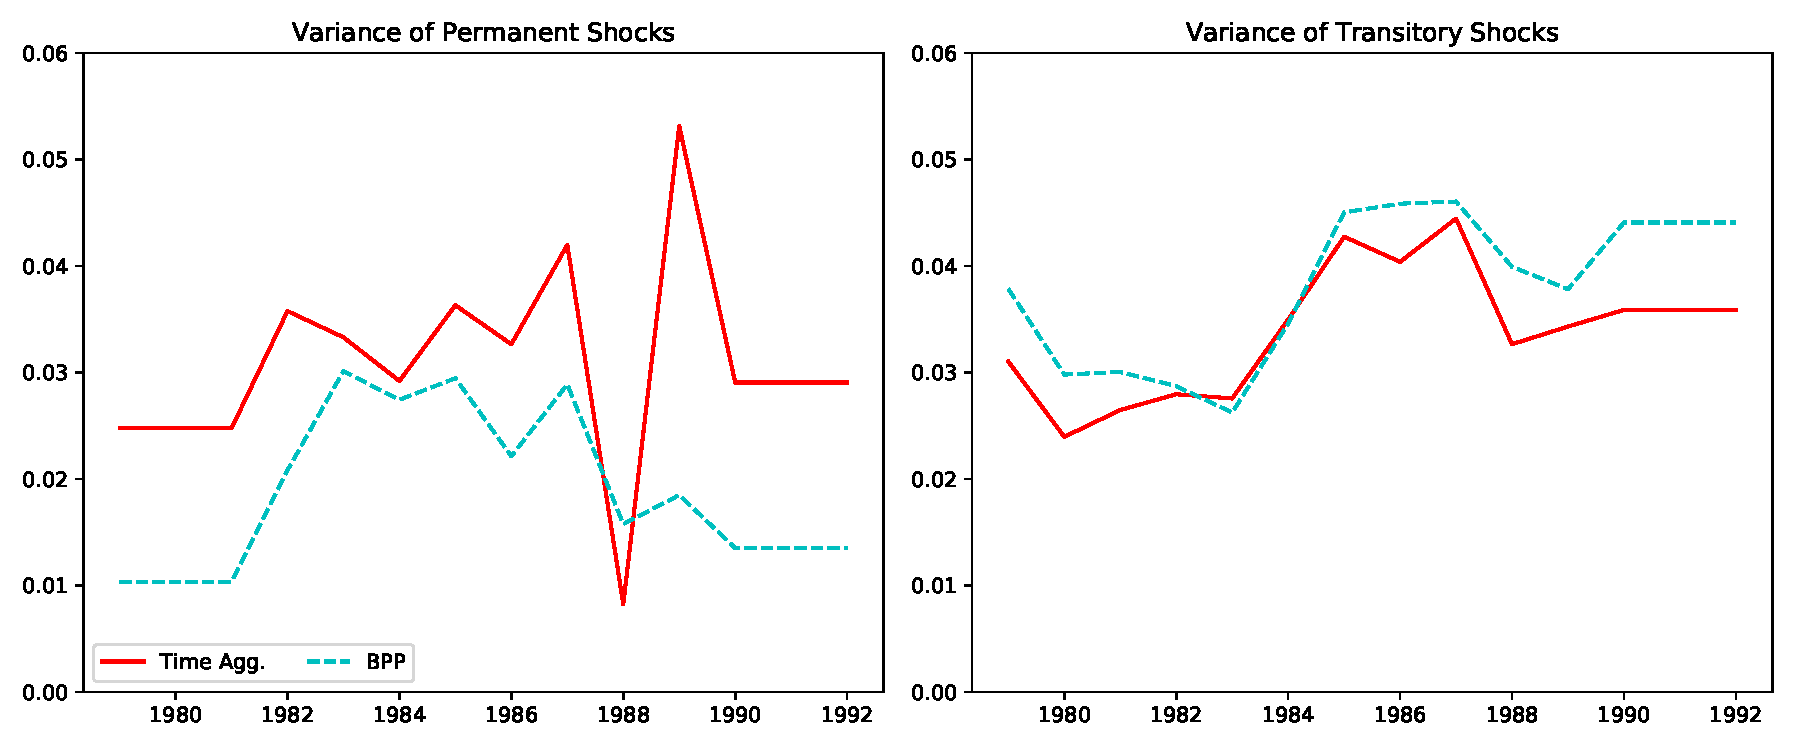
\includegraphics[width=1\textwidth]{./Chapter1/Figures/ShockVariances1980s.pdf}
	\footnotesize Notes: BPP plots the variances from Table 6 of the original BPP paper. Time Agg. plots the equivalent variances corrected for the time aggregation problem.
\end{figure}

\section{Conclusion}
This paper highlights the importance of time aggregation when working with panel data, especially when analyzing the covariance matrix of income and consumption growth. It also resolves the dissonance between BPP's estimates of transitory income insurance and the natural experiment literature on marginal propensity to consume. Going forward I hope the methods used here to correct for the time aggregation problem can be useful for researchers, especially as more and more high quality panel datasets on income and consumption become available.

%\processdelayedfloats

%\small
%\bibliography{AllPapers}
%\normalsize

\pagebreak
%\appendix

\section*{Appendix}
\input ./Chapter1/AppendixLevelvsLogs.tex
\input ./Chapter1/AppendixFullMoments.tex
\input ./Chapter1/AppendixTransitoryPersistence.tex
\input ./Chapter1/AppendixTypicalWeek.tex

\section{Other Tables from the BPP paper} \label{table_appendix}
Table \ref{table:ReplicationTable7} replicates Table 7 from the original BPP paper.

\input ./Chapter1/Tables/RepTable7.tex 

Table \ref{table:ReplicationTable8} replicates Table 8 from the original BPP paper.\input ./Chapter1/Tables/RepTable8.tex









%\include{chapter2}
%\include{chapter3}


%% REFERENCES

% if you use BIBTEX
%\bibliographystyle{econometrica}
%\bibliographystyle{IEEEtran}
%\bibliography{Reference_new}


%\begin{vita}
%
%\begin{wrapfigure}{l}{0pt}
%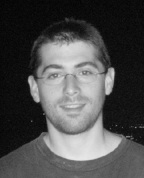
\includegraphics[width=2in,height=2.5in,clip,keepaspectratio]{rjvheadshot}
%\end{wrapfigure}
%
%\end{vita}
\end{document}
